\documentclass[format=acmsmall, review=false, screen=true]{acmart}

\usepackage{booktabs} % For formal tables

\usepackage[ruled]{algorithm2e} % For algorithms
\renewcommand{\algorithmcfname}{ALGORITHM}
\SetAlFnt{\small}
\SetAlCapFnt{\small}
\SetAlCapNameFnt{\small}
\SetAlCapHSkip{0pt}
\IncMargin{-\parindent}


% Metadata Information
\acmJournal{TWEB}
\acmVolume{9}
\acmNumber{4}
\acmArticle{39}
\acmYear{2010}
\acmMonth{3}
\copyrightyear{2009}
%\acmArticleSeq{9}

% Copyright
%\setcopyright{acmcopyright}
\setcopyright{acmlicensed}
%\setcopyright{rightsretained}
%\setcopyright{usgov}
%\setcopyright{usgovmixed}
%\setcopyright{cagov}
%\setcopyright{cagovmixed}

% DOI
\acmDOI{0000001.0000001}

% Paper history
\received{February 2007}
\received[revised]{March 2009}
\received[accepted]{June 2009}


% Document starts
\begin{document}
% Title portion. Note the short title for running heads
\title[Edge2photo]{A Multifrequency MAC
  Specially Designed for Wireless Sensor  Network Applications}

\author{Yuhang Li}
%\orcid{1234-5678-9012-3456}
\affiliation{%
  \institution{University of Science and Technology of China}
  \streetaddress{xx Rd}
  \city{Hefei}
  \state{Anhui}
  \postcode{230027}
  \country{China}}
\email{lyh9001@mail.ustc.edu.cn}
\author{Xuejin Chen}
\affiliation{%
  \institution{University of Science and Technology of China}
  \streetaddress{xx Rd}
  \city{Hefei}
  \state{Anhui}
  \postcode{230027}
  \country{China}
}
\email{xjchen99@ustc.edu.cn}



\begin{abstract}
This is an abstract example of this Latex template.<<<<
Multifrequency media access control has been well understood in
general wireless ad hoc networks, while in wireless sensor networks,
researchers still focus on single frequency solutions. In wireless
sensor networks, each device is typically equipped with a single
radio transceiver and applications adopt much smaller packet sizes
compared to those in general wireless ad hoc networks. Hence, the
multifrequency MAC protocols proposed for general wireless ad hoc
networks are not suitable for wireless sensor network applications,
which we further demonstrate through our simulation experiments. In
this article, we propose MMSN, which takes advantage of
multifrequency availability while, at the same time, takes into
consideration the restrictions of wireless sensor networks. Through
extensive experiments, MMSN exhibits the prominent ability to utilize
parallel transmissions among neighboring nodes.>>>>
\end{abstract}


%
% The code below should be generated by the tool at
% http://dl.acm.org/ccs.cfm
% Please copy and paste the code instead of the example below.
%
\begin{CCSXML}
<ccs2012>
 <concept>
  <concept_id>10010520.10010553.10010562</concept_id>
  <concept_desc>Computer systems organization~Embedded systems</concept_desc>
  <concept_significance>500</concept_significance>
 </concept>
 <concept>
  <concept_id>10010520.10010575.10010755</concept_id>
  <concept_desc>Computer systems organization~Redundancy</concept_desc>
  <concept_significance>300</concept_significance>
 </concept>
 <concept>
  <concept_id>10010520.10010553.10010554</concept_id>
  <concept_desc>Computer systems organization~Robotics</concept_desc>
  <concept_significance>100</concept_significance>
 </concept>
 <concept>
  <concept_id>10003033.10003083.10003095</concept_id>
  <concept_desc>Networks~Network reliability</concept_desc>
  <concept_significance>100</concept_significance>
 </concept>
</ccs2012>
\end{CCSXML}

\ccsdesc[500]{Computer systems organization~Embedded systems}
\ccsdesc[300]{Computer systems organization~Redundancy}
\ccsdesc{Computer systems organization~Robotics}
\ccsdesc[100]{Networks~Network reliability}

%
% End generated code
%


\keywords{Generative adversarial nets, edge maps, realistic images}




\maketitle

% The default list of authors is too long for headers.
\renewcommand{\shortauthors}{Y. Li and X. Chen}

%\input{samplebody-journals}
\section{Introduction}
% emphasize the chanllenges of edge2face!
Realistic image synthesis has been a hot topic in computer vision and computer graphics for years. 
Traditional methods \cite{EBSR, TextureSyn,SceneCompletion} establish databases of existing images, and generate images by matching and merging images in the database patch-wisely. 
With the emergence of deep neural networks (DNN), several promising DNN-bsed approaches for image synthesis have been proposed. 
Variational autoencoders (VAEs) \cite{VAEs}, which maximize a variational lower bound on the log-likelihood of the training data, have brought some progress in generating visually plausible images, but the generated samples suffer from being blurry. 
Autoregressive models \cite{PixelCNN} generate image pixel by pixel and are able to generate convincing samples. However, it is computational inefficient to sample images from these models.
%

Generative adversarial networks (GANs) \cite{GANs} offer a new and promising mechanism to generate images, which take noise vectors as input and train two networks playing minmax game to guide the generated samples to be indistinguishable from the real ones. 
Conditional GANs, which generate image from assigned conditional information instead of noise vector, are conditional versions of GANs. Conditional GANs are trained in a supervised manner and shown to be powerful in modeling the conditional distributions with respect to the assigned conditions. A variety of conditions have been applied to conditional GANs, such as discrete class labels \cite{cGANs}, texts \cite{StackGANs, StackGANs++}, and images.
%
Among these conditional image generation methods, image-to-image translation has drawn a lot of attention recently, which aims to apply a conditional image in one domain to generate the corresponding target image in another, reserving shared concepts, objects or scenes in these two images. Since the first image-to-image model (pix2pix)  \cite{pix2pix} was proposed, there have been many variants of this approach in both supervised and unsupervised manner \cite{CycleGANs, DualGANs,CoupleGANs,BicycleGANs}. 
However, the pix2pix model has troubles in some cases of translating face images from the corresponding edge maps. For example, the convolutional-based pix2pix model fails to render a well-defined part, such as an eye, in the generated image if the conditional edge map does not contain such information. The reasons behind this might be two-folded.
%
1)Since the convolution operator has a local receptive field depending on the size of its kernels, a large receptive field is achieved by cooperation of several convolution layers. It is hard for the optimizer to discover parameter values that model the long-range dependencies through several convolutional layers \cite{SAGANs}. 
2) The discriminator used in the pix2pix model \cite{pix2pix} focuses on examining local patches instead of capturing the global information, and therefore fails to guide the generator to synthesize the global structure of the conditional image. 

Considering the first reason, we introduce a conditional self-attention mechanism to the generator of image-to-image models to address the problem.
Self-attention \cite{Non-local, Attention, MachineReading, SAGANs}, which computes the response at a position as a weighted sum of the features at all positions, is able to capture the long-range dependencies across different regions of images and feature maps. In order to adapting the conditional setting of image-to-image translation and encouraging the model to leverage the information of the conditional image directly, we propose a conditional self-attention module (CSAM) which enables the higher layers to sense the conditional image. 
%
For the second reason, we consider to establish multiple discriminators to capture information of different levels, both patch-wisely and globally. We note that similar idea of multiple discriminators has been raised by \cite{LaplaceGANs, SGANs, StackGANs, CRN} who resizes the real/fake samples and applies multiple discriminators to these multi-scale samples. 

In this research, we propose Conditional Self-attention Generative Adversarial Networks (SCGANs), which translate images from one domain to another being able to capture long-range dependencies and reserve the global structures. With the help of the novel CSAMs, the conditional image is able to guide the higher layers in the architecture directly.  

Our contributions are summarized as follow:

i) We firstly introduce the self-attention mechanism to image-to-image translation and propose a novel conditional self-attention generative adversarial networks for the image-to-image translation task. Unlike convolutional-based methods, the proposed model is able to model the long-range dependencies and global structure across images.

ii)

iii)

The rest of this article is organized as follow. Related works are presented in Section \ref{sec:related_work}. The method we proposed is introduced in Section \ref{sec:method}. We demonstrate the effectiveness of method by experiments in Section \ref{sec:experiment}. Section \ref{sec:conclusion} summarizes our conclusions and outlines 
possible future work.
\section{Related work}
Our work is based on generative adversarial networks (GANs)~\cite{GAN} in a conditional setting. In this section, we present related research in GANs.
\subsection{Generative Adversarial Networks}
Generative adversarial networks (GANs) \cite{GANs} have obtained a great success in recent years.
A classical architecture of GANs contains a generator network and a discriminator network. The task of the generator take a noise vector as input and generate samples indistinguishable from the real ones, while the discriminator, in opposite, attempt to find out whether its input is real or synthesized. The minmax game played by these two networks guides the generated distribution to be similar to the real data distribution. 
%
Many recent works extent GANs to a wide range of applications, such as image generation [1, 42, 62], representation learning [45], image manipulation [64], object detection [33], and video applications [38, 51, 54]. 

\subsection{Conditional Generative Adversarial Networks}
Conditional GANs were firstly introduced by \cite{CGAN} who treated the conditional generation problem as the inverse processing of image classification and used discrete labels as condition to generate images. Previous works have explored GANs generating images in the condition of discrete labels~\cite{CGAN}, text~\cite{Reed2016} and images.
%
\cite{Dosovitskiy2014} trained convolutional networks to generate images of objects given object style, viewpoint and color. With the experiments of interpolating viewpoints, they showed that networks learn a meaningful representation of 3D models. 
%
\cite{Reed2016} generated photo-realistic images conditioned on text descriptions. 
%
Our work utilize GANs in a conditional setting to generate images from images.


\subsection{Image-to-image translation with GANs}
Given an image in one domain, image-to-image translation methods generate a corresponding image in another. These two images are possible representations of the same scene or object. Image-to-image translation with GANs is a special case of conditional GANs where images are applied to be conditions. 
%

\cite{pix2pix}, called pix2pix, firstly introduced the concept of image-to-image translation, who treated one image in a paired image dataset as conditioned input and generate its corresponding image. 
%Unlike prior works which dealt with only one application, \cite{pix2pix} are able to handle multiple applications in one frame work only switching training datasets. 
Pix2pix applies skip connections \cite{Unet} between mirrored layers in the generator to make sure low-level information pass through its encoder-decoder architecture and uses patch discriminators \cite{PatchDicriminator} to increase the performance of the generator. >>>Discuss the shortage of pix2pix<<<
%
\cite{UNIT} studied on unpaired image-to-image translation by training a two-branch GAN. Each branch is composed with a encoder, a generator and a discriminator. With the idea that high-level representation of a pair of corresponding images in two domains should be the same, high-level layers share weights between two branches in encoders, generators and discriminators. 
%
CycleGAN~\cite{CycleGAN}, DiscoGAN~\cite{DiscoGAN} and DualGAN~\cite{DualGAN} developed similar architectures to translate unpaired images which contain, for each, two generators and two discriminators. These methods learn two mappings in an adversarial training process such that an input image in one domain is mapped to a generated image in another, and then the generated image is mapped to a reconstructed image which is closed to the input image in some measures. These methods shared the same idea that since the generated image is able to reconstruct the input image, it should contain the content of the input image. >>>>discuss the different between supervised and unsupervised methods<<<<<

\subsection{Attention mechinism}
>>>>>> Not familiar yet. <<<<<<<<<
\section{Method}
\label{sec:method}

%
\begin{figure}
	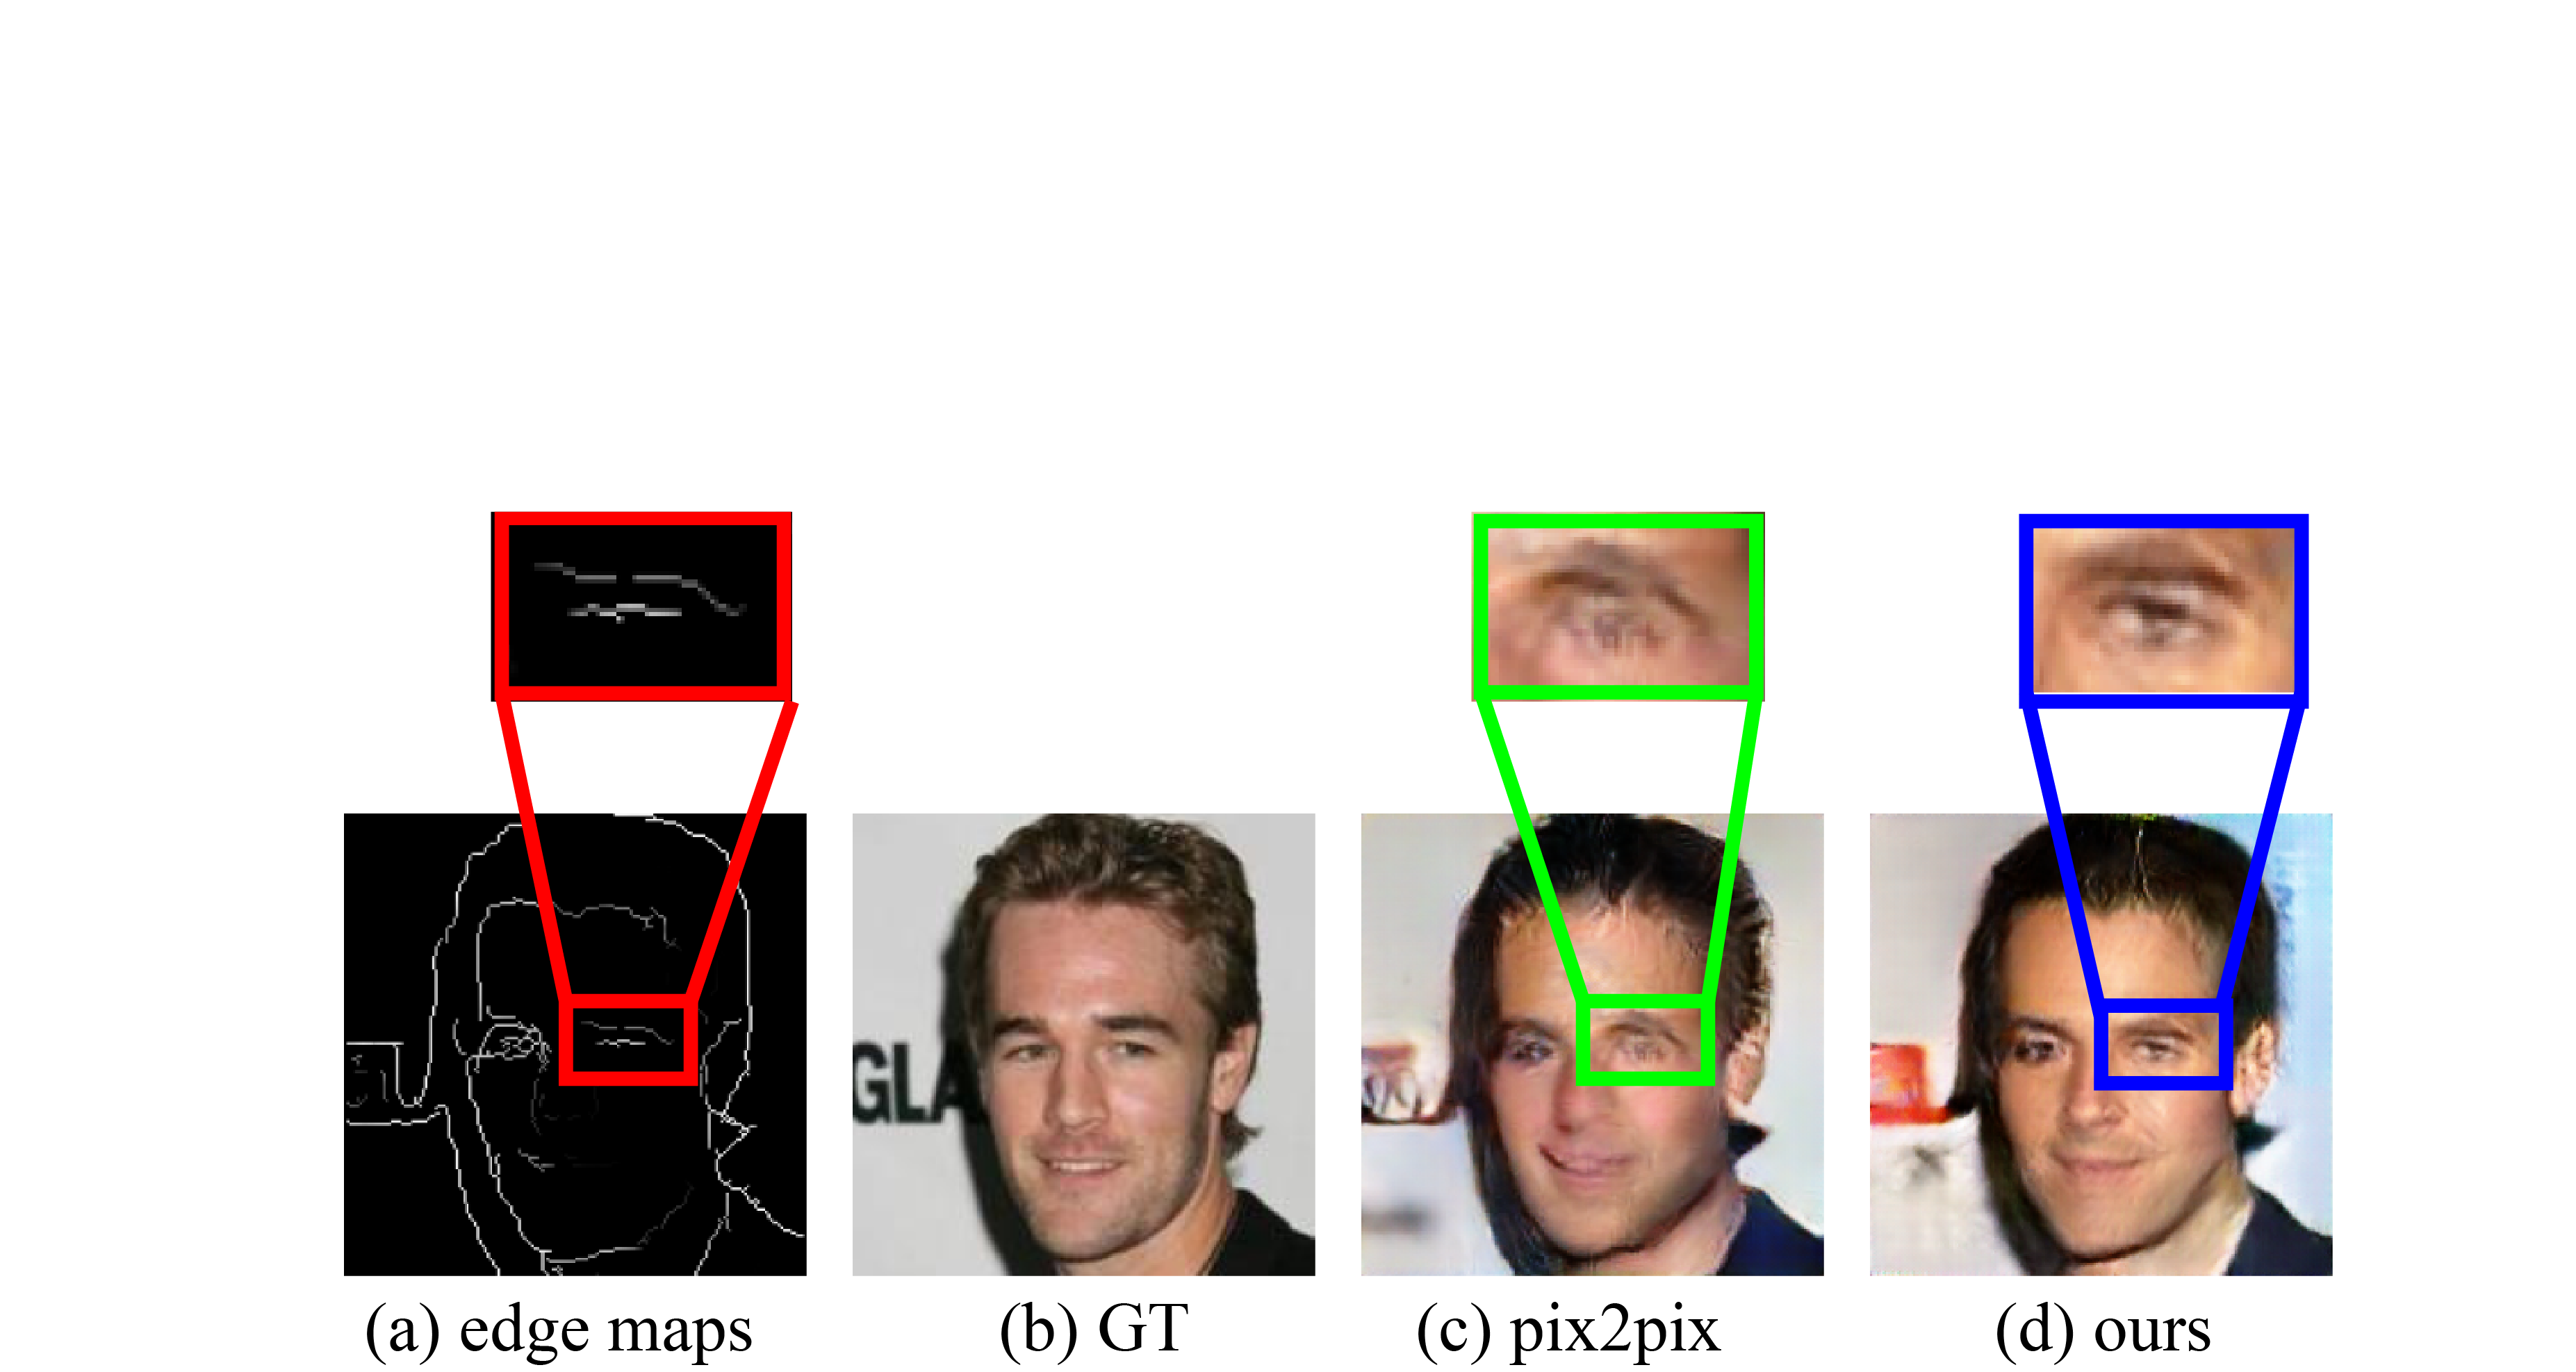
\includegraphics[width=0.8\textwidth]{figures/example}
	\caption{An example of translating face images (b) from the corresponding edge maps (a). In this example, the edge map does not contain the complete edges of the left eye (on the right hand side of the reader). It is obvious that there should be a left eye in the red square according to the global structural information. The pix2pix model (c) fails to render a recognizable eye in the corresponding location (green square) while the proposed method (d) is able to generate the entire structure even when the conditional edge map lacks several parts of the global structure.}
	\label{fig:example}
\end{figure}
%
% too many "long-range dependencies"
The proposed Conditional Self-attention Generative Adversarial Networks (CSAGANs), which translate images from one domain to another and are able to capture long-range dependencies and reserve the global structures across image. We first review the pix2pix model as our baseline (Sec.\ref{subsec:pix2pix}). And then we introduce the Conditional Self-attention Module (SCAM) (Sec. \ref{subsec:CSAM}). Finally, we describe the idea of multiple level patch discriminator (Sec.\ref{subsec:disciminator} and the architecture we proposed (Sec. \ref{subsec:architecture}).
\subsection{The Pix2pix Model}
\label{subsec:pix2pix}
Since our model is based on the pix2pix model \cite{pix2pix}, we review this model in this sub-section. The pix2pix model is an image-to-image translation framework based on conditional GANs, which trains a generator network $G$ and a discriminator network $D$ alternatively. The generator $G$ takes a conditional image as input and outputs the corresponding target image, while the discriminator $D$ distinguishes real images from the synthesized ones. To train these two networks in a supervise manner, a set of corresponding image pairs $\{(\bm{x}_i, \bm{y}_i)\}$ is required as training set, where $\bm{x}_i$ is a conditional image and $\bm{y}_i$ is the corresponding target image. These two networks play a minmax game to guide the generator to model the conditional distribution of real images given the conditional images. The objective is given by:
\begin{equation}
\label{eqn:minmax_game}
\min_G \max_D \mathcal{L}_{adv}(G,D)+\lambda \mathcal{L}_{L1}(G),
\end{equation}
where $G$ aims to minimize this objective while $D$ tries to maximize it inversely.
The adversarial loss function is generally given by 
\begin{equation}
\label{eqn:loss_adv}
\mathcal{L}_{adv}(G,D)=E_{(\bm{x},\bm{y})\sim p_{data}(\bm{x},\bm{y})}[\log D(\bm{x},\bm{y})]+E_{\bm{x}\sim p_{data}(\bm{x})}[\log(1-D(\bm{x},G(\bm{x})))],
\end{equation}
and the $L_1$ loss is given by
\begin{equation}
\label{eqn:loss_l1}
\mathcal{L}_{L1}(G)=\mathbb{E}_{(\bm{x},\bm{y})\sim p_{data}(\bm{x},\bm{y})}[\|\bm{y}-G(\bm{x})\|_1]
\end{equation}
The generator of the pix2pix model is a fully-convolution-based U-Net \cite{Unet}. The input of the generator is only applied to the first layer. The discriminator of the pix2pix model is a patch-wise discriminator, which examines only a patch of its input image and uses the average of outputs from all patches of the input image as the ultimate output. The size of each patch is set to $70\times 70$. The conditional image is concatenated channel-wisely to the synthesized image or real image as the input of the discriminator. 

However, in the task of translating a face image from the corresponding edge map, the pix2pix model has troubles to generate realistic face images in some cases with structural constrains. Since faces have well-defined structural parts, e.g. noses, mouths, eyes and etc., the synthesized face images should contain the whole set of these structural part to be realistic, even when the conditional edge maps lack of edges on the supposed locations of these parts. The pix2pix fails to generate realistic structural part in this circumstance.
% take the first low of the result figure as example
An example is displayed in Figure \ref{fig:example}. In this example, an edge map of a face, shown on the left of the figure, only captures a part of edges of the left eye (in the green square) rather than the whole set of edges of the entire left eye. The face image generated by the pix2pix model on the condition of this edge map is shown on the right in the figure. According to the global structural information, there should be a left eye in the red square obviously. However, we can observe that the pix2pix model fails to render a recognizable left eye in the synthesized face image. 

This phenomenon might be caused by two reasons. 
1) The pix2pix model is a convolution-based model which relies on convolutional operations to model the dependencies across different regions of images and feature maps. Convolutional operations have local receptive fields depending on the kernel sizes and are not able to balance between ability to model long-range dependencies and efficiency of computation and statistics in some cases \cite{SAGANs}.
2) The discriminator used by the pix2pix model is patch-wised, based on the assumption that pixels separated by a distance more than a patch diameter are independent to each other. This assumption is true in some cases like texture generation and style transfer, and has been applied in previous work \cite{texture_markovian, styel_transfer}. However, this assumption fails in the case with global structural constrains. Therefore the patch-wise discriminator fails to grasp the global structure information and is not able to guide the generator to be aware of the structure of the faces.

To address the problem caused by the first reason, we introduce self-attention to the generator of image-to-image models to address the problem.
Self-attention \cite{Non-local, Attention, MachineReading, SAGANs}, which computes the response at a position as a weighted sum of the features at all positions, is able to capture the long-range dependencies across different regions of images and feature maps. In order to adapting the conditional setting of image-to-image translation and encouraging the model to leverage the information of the conditional image directly, we propose a conditional self-attention module (CSAM), which enables the higher layers to sense the conditional image, as a general module of networks.
%
For the second reason, we consider to establish a multi-level discriminator to capture the information of its input image both patch-wisely and globally. We note that similar ideas of multiple discriminators have been raised by \cite{LaplaceGANs, SGANs, StackGANs, CRN} with different architectures. We describe CSAM and the multi-level discriminator in next sections.
%
%
\begin{figure}
	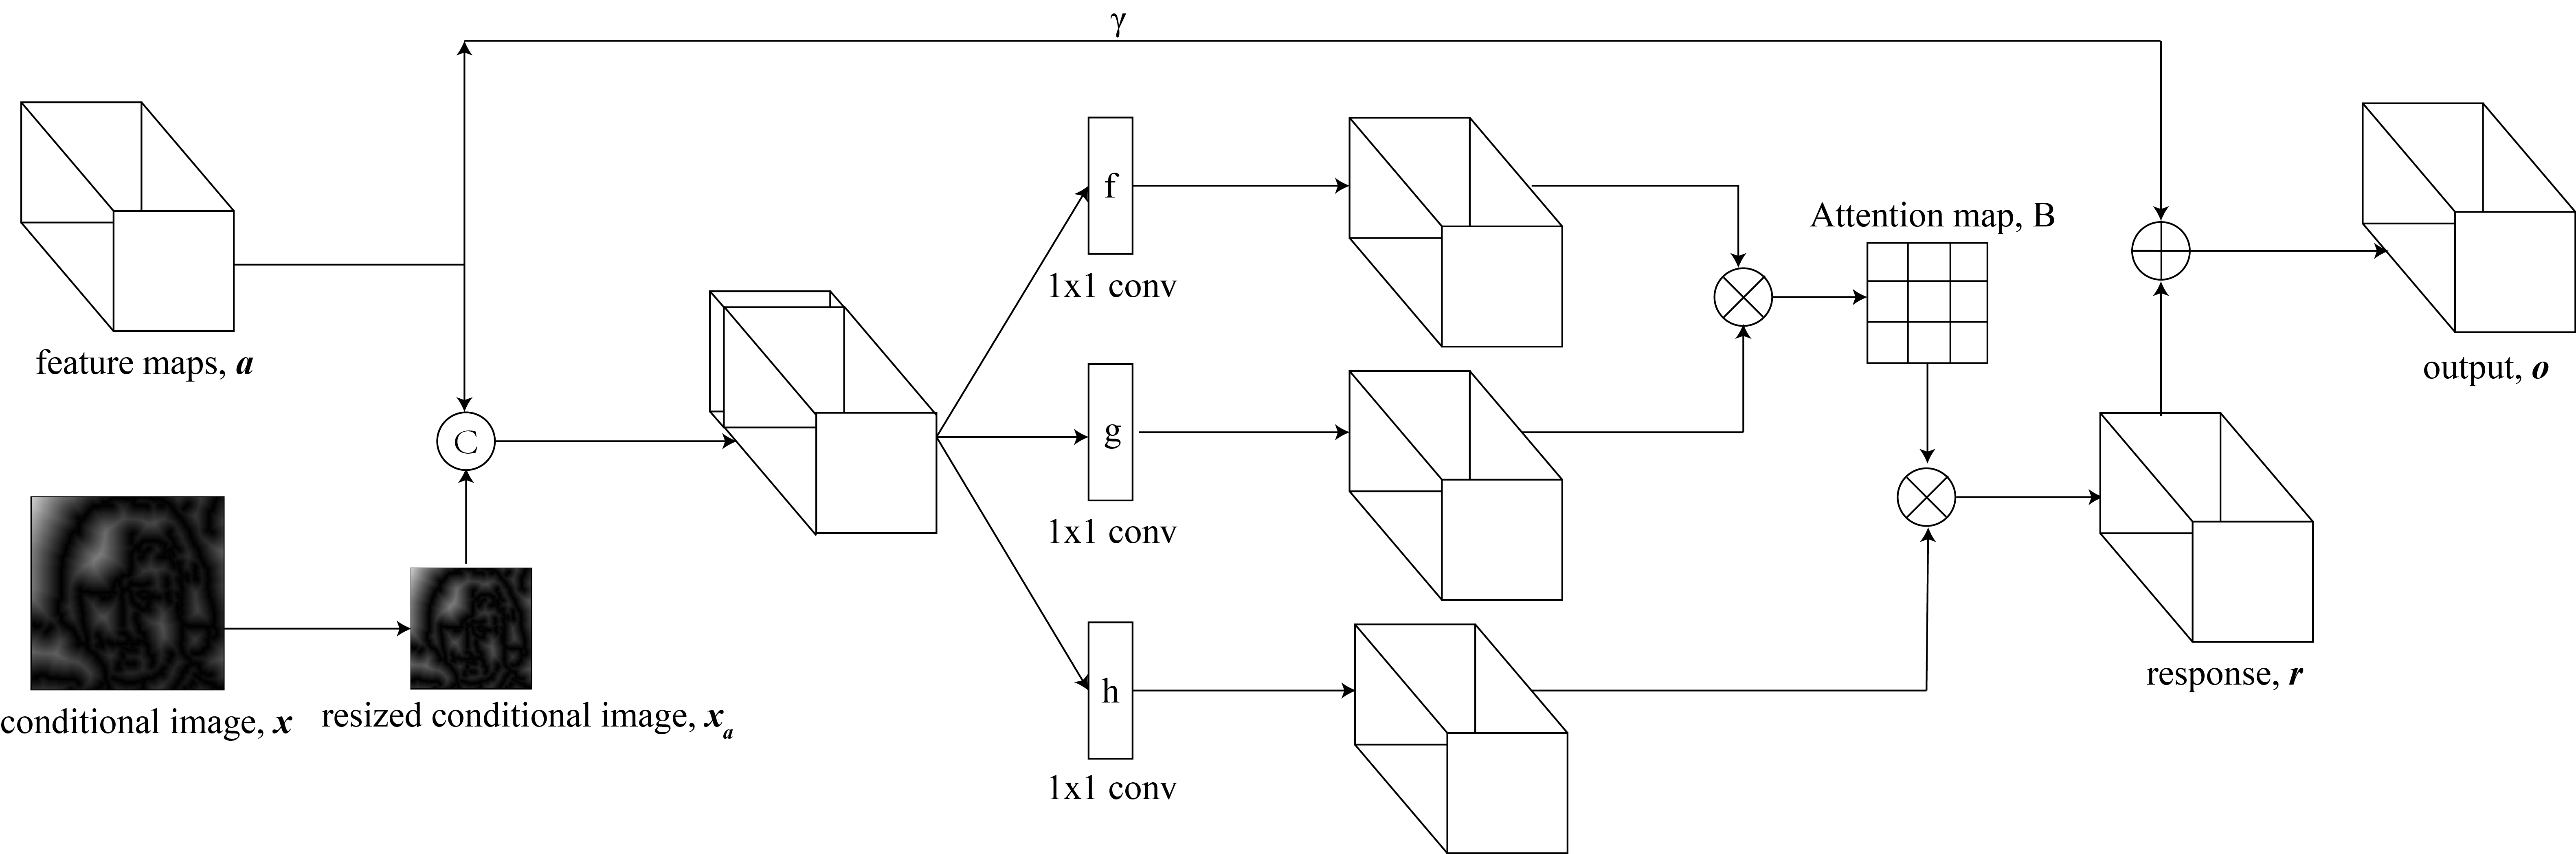
\includegraphics[width=\textwidth]{figures/CSAM}
	\caption{The proposed CSAM. Given the conditional image and feature maps from the previous layer, the output feature maps are calculated in a self-attention manner. This module is designed to be added after any assigned layers.}
	\label{fig:CSAM}
\end{figure}
%
%
\subsection{Conditional Self-Attention Module (CSAM)}
\label{subsec:CSAM}
We improve the pix2pix model by utilizing self-attention mechanism to capture the long-range dependencies of images and feature maps. A recently proposed method \cite{SAGANs} has introduced self-attention to unconditional GANs and achieved state-of-the-art results. Inspired by this method, we propose a conditional self-attention module (CSAM) which is suitable for image-to-image translation framework and able to leverage the conditional information directly. This module is designed as a general module of conditional frameworks and can be added after any existing modules. We will provide details of our architecture in Subsection \ref{subsec:architecture}. The formulation of CSAM is described below.

% $\boldmath{x} \bold{x} \mathbf{x} \mathbm{x} \vec{x}$
% TODO: notation of vectors and matrices, images and feature maps 
Given the conditional image $\bm{x}\in \mathbb{R}^{3\times N_{\bm{x}}}$ and feature maps from the previous layer $\bm{a}\in \mathbb{R}^{C\times N_{\bm{a}}}$, we first resize the conditional image $\bm{x}$ to match the size of $\bm{a}$ and get $\bm{x}_{\bm{a}}\in \mathbb{R}^{3\times N_{\bm{a}}}$. Here $N_{\bm{x}}=H_{\bm{x}}\times W_{\bm{x}}$, where $H_{\bm{x}}, W_{\bm{x}}$ are the height and width of the conditional image $\bm{x}$. $N_{\bm{a}}$ is defined similarly for $\bm{a}$.
Then we concatenate the resized conditional image $\bm{x}_{\bm{a}}$ to the feature maps $\bm{a}$ to get $[\bm{a}, \bm{x}_{\bm{a}}]$ as conditioned features, where $[\cdot,\cdot]$ is the concatenation operation. This allows the information of conditional image to convey to every attention module and guide the network to form the attention directly based on the conditional image.
%

In order to calculate the attention, we map the conditional features $[\bm{a}, \bm{x}_{\bm{a}}]$ to two feature spaces by:
\begin{equation}
\label{eqn:f}
f([\bm{a}, \bm{x}_{\bm{a}} ])=\mathbf{W}_f[\bm{a}, \bm{x}_{\bm{a}} ],
\end{equation}
\begin{equation}
\label{eqn:g}
g([\bm{a}, \bm{x}_{\bm{a}} ])=\mathbf{W}_g[\bm{a}, \bm{x}_{\bm{a}} ],
\end{equation}
where $W_f, W_g\in \mathbb{R}^{\hat{C}\times (C+3)}$ are trainable weights and are implemented by $1\times 1$ convolutions. Here, we use $\hat{C}=C/8$ in our experiments following the setting of previous work \cite{SAGANs}.
%
Let $\mathbf{B}\in \mathcal{R}^{N_{\bm{a}}\times N_{\bm{a}}}$ be the attention map. Every element in $\mathbf{B}$ is denoted as $b_{j,i}$ which indicates the extent to which the model attends to the $i^{th}$ location when synthesizing the $j^{th}$ region and is calculated by 
\begin{equation}
\label{eqn:beta}
b_{j,i}=\frac{exp(s_{ij})}{\sum^{N_a}_{i=1}exp(s_{ij})}
\end{equation}
where $s_{ij}=f([\bm{a}, \bm{x}_{\bm{a}} ])^Tg([\bm{a}, \bm{x}_{\bm{a}} ])$. Next, we use $b_{j,i}$ as the attention weights and compute the response $\bm{r}=(\bm{r}_1, \bm{r}_2,\cdots, \bm{r}_{N_{\bm{a}}})\in \mathbb{R}^{C\times N_{\bm{a}}}$ at every position as a weighted sum of the features at all positions, where
\begin{equation}
\label{eqn:response}
\bm{r}_j=\sum^{N_{\bm{a}}}_{i=1}b_{j,i}h([\bm{a}, \bm{x}_{\bm{a}} ]),
\end{equation}
where $h([\bm{a}, \bm{x}_{\bm{a}}])=\mathbf{W}_h[\bm{a}, \bm{x}_{\bm{a}} ]$ and $\mathbf{W}_h\in \mathbb{R}^{(C+3)\times (C+3)}$.
As suggested in \cite{SAGANs}, we further multiply the response of the attention layer by a scale parameter $\gamma$ and add back to the input feature maps. The final output is calculated by 
\begin{equation}
\label{eqn:output}
\bm{o}_i=\gamma \bm{r}_i+\bm{a}_i,
\end{equation}
where $\gamma$ is trainable value and is set to $0$ at the beginning of the training process. This is because at the early stage of training process, the networks are able to learn the local dependencies, and then learn the long-range dependencies by assign more weight to the non-local evidence progressively.
%
%
\subsection{Multi-Level Patch Discriminator}
\label{subsec:disciminator}
The discriminator of the pix2pix model is patch-wised, which distinguishes the real/synthesized images patch by patch convolutionally with in a local receptive field much smaller than the size of the input images. 
The average value of all responses is provided as the ultimate output of $d$. 
This is based on the assumption of independence between pixels separated by more than a patch diameter. 
However, since the structural constrain is global information across the entire image, the patch-wise discriminator lacks ability to capture this global information.
We add another global discriminator $D_g$ with a receptive field as large as the entire image to capture the global structure information. The patch discriminator $D_p$ and the global discriminator $D_g$ share weights in first few layers since the lower features of these discriminators should be the same, as shown in Figure \ref{fig:architecture}. The objective of the minmax game therefore is modified from Equation \ref{eqn:minmax_game} to
\begin{equation}
\label{eqn:new_minmax_game}
\min_G \max_{D_g, D_p} \mathcal{L}_{adv}(G;D_g,D_p)+\lambda \mathcal{L}_{L1}(G),
\end{equation}
where the adversarial loss is given by 
\begin{equation}
\label{eqn:new_loss_adv}
	\begin{aligned}
	\mathcal{L}_{adv}(G;D_g,D_p)&=E_{(\bm{x},\bm{y})\sim p_{data}(\bm{x},\bm{y})}[\log D_g(\bm{x},\bm{y})+\log D_p(\bm{x},\bm{y})] \\
	&+E_{\bm{x}\sim p_{data}(\bm{x})}[\log(1-D_g(\bm{x},G(\bm{x})))+\log(1-D_p(\bm{x},G(\bm{x})))],
	\end{aligned}
\end{equation}
and $L_1$ loss is still the same as Equation \ref{eqn:loss_l1}.
%
%
\subsection{Architecture}
\label{subsec:architecture}
% add CSAMs to discriminator or not? if not, why? (GPU memory budget limited)
Our architecture, shown in Figure \ref{fig:architecture}, is based on that of the pix2pix method which uses a convolution-based U-Net \cite{Unet} as its generator and a patch-wise discriminator. We add a proposed CSAM after every convolutional layer of the generator except the first and last ones. The conditional image is resized to specific size and concatenate to the previous feature maps as the input of every CSAM. CSAMs are able to access the information of the conditional image directly and model the long-range dependencies across images and feature maps. Also, we switch the patch-wise discriminator into the proposed multiple level patch discriminator to enable the discriminator network to capture both global and local information and therefore guide the generator to generate images with more structural layout. More details of the architecture are discussed below.
%
\begin{figure}
	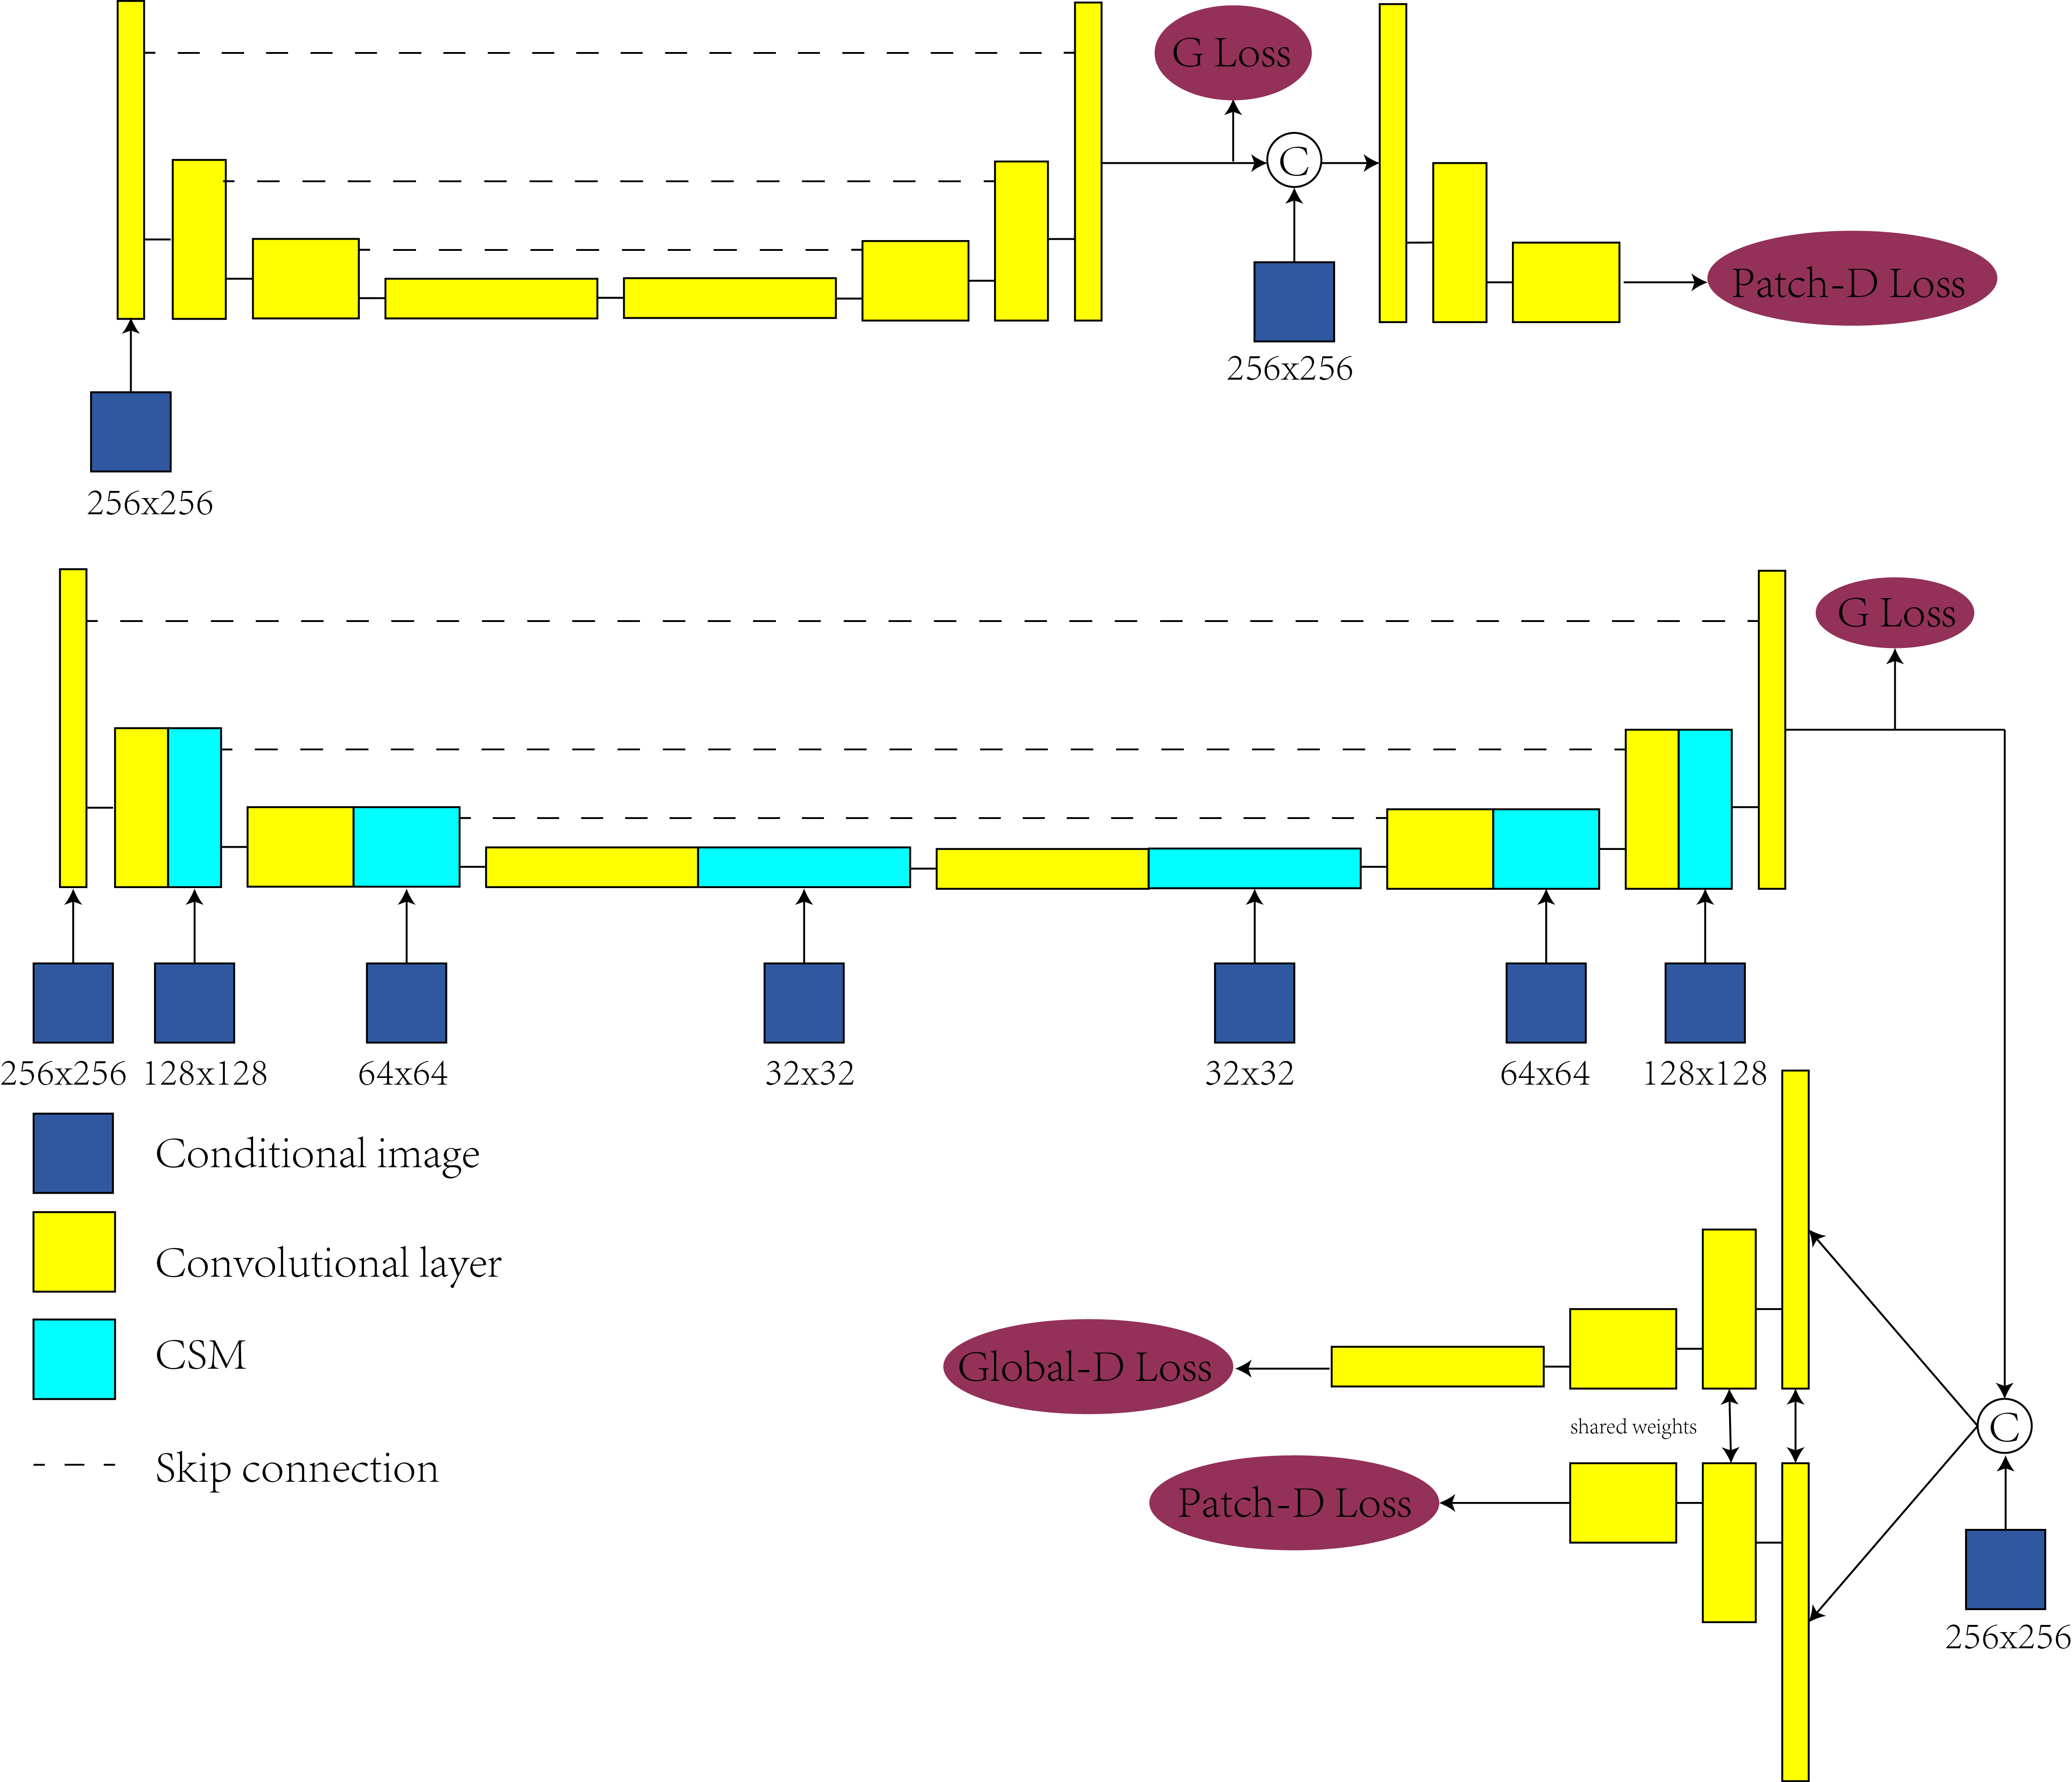
\includegraphics[width=0.8\textwidth]{figures/architecture}
	\caption{The pix2pix framework (the upper architecture) and the proposed framework (the lower architecture). Compared to the pix2pix model, in the generator of CSAGAN CSAMs are added after every convolutional layers except the first and the last ones. The discriminator is changed into a multi-level discriminator. The conditional image is resized and connect to every CSAM in the generator.}
	\label{fig:architecture}
\end{figure}
%
%
\paragraph{Noise vector} Some past conditional GANs add a noise vector to the generator as input to avoid it producing a deterministic output. However, the pix2pix model has shown that the noise vector is just ignored by the generator network and hardly change the output samples. We observe the same phenomenon in our experiments and do not apply the noise vector in our model. 
\paragraph{Spectral Normalization} Spectral normalization \cite{SN} is a recently proposed normalization technique, which restricts the spectral norm of each layer of the discriminator to constrain its Lipschitz constant. Spectral normalization is computationally efficient and require no extra hyper-parameter. It has shown that spectral normalization also benefit the training of generator by avoiding unusual gradients. We add spectral normalization to the discriminator and CSAMs in the generator.
%
\section{Experiment}
\label{sec:experiment}
We propose the CSGANs framework, which translate images from one domain to another, being able to capture long range dependencies and reserve the global structures. To demonstrate the effectiveness of our framework, we have performed several experiments. In this section, we discuss 
\subsection{Implementation Details}
In order to comparing with the pix2pix model, we basically follow its implementation details. We use minibatch SGD and Adam \cite{Adam} optimizer with learning rate $lr=0.002$ and momentum parameters $\beta_1=0.5, \beta_2=0.999$. We update one step for either of $G$ and $D$ alternatively. Batch normalization is used in convolutional layers of the generator. Batch size is set to 8.
\subsection{Dataset}
We evaluation our method with the task of translating edge maps to natural images, e.g. the target images are face images while the conditional images are the corresponding edge maps. The face images of the dataset we used are face images of CelebA dataset \cite{CelebA}, which  is a large-scale face attributes dataset with more than 200K celebrity images. Faces have well-defined structure of eyes, noses, mouths, and etc., and therefore the artifacts are visually sensitive for observers. This makes face images suitable for evaluating the proposed method.  We utilize the cropped and aligned version of dataset with the size of every images being $218\times 178$. In order to meat the original setting of the pix2pix method, we center-crop the images and resize the image to $256\times 256$ in both experiments of the pix2pix model and the proposed model. The face attributes are attached in the dataset but not included in our experiments. 

The edge maps we use generated in the pipeline similar to that used in pix2pix paper. Specifically, the edges are firstly extracted using a deep edge detector named holistically-nested edge detect (HED) \cite{HED}. We keep the values of each edge pixels calculated by HED in the edge maps. Each of these values is supposed to indicate the probability of being edge in the positions of pixel. And then several steps of post-processing are conducted to obtain simpler and clearer edge maps with fewer edge fragments, including thinning, short edge removal, and erosion. In addition, since the edge maps are very sparse, we add one more step to the process to decrease the sparsity of edge maps. We calculate an unsigned euclidean distance field for each edge map to obtain a dense representation. We note that similar idea of distance filed representations can be found in some recent works \cite{repair_3d, shape_completion, SketchyGANs}. In Section \ref{subsec:ablation}, we will prove the advantages of distance fields by experiments.

%
%
\subsection{ Evaluation Metrics}
The evaluation of generative models is an open and complicated task, because a model with good performance with respect to one criterion need not imply good performances with respect to the other criteria \cite{evaluation, GANs_equal}. Traditional metrics, such as pixel-wise mean-squared error do not present the joint statistics of the synthesized samples and therefore is not able to evaluation the performance to a conditional generated model. 
Inception Score (IS) \cite{IS} is a widely-used criterion. However, IS has been pointed out to have serious limitations that it focuses more on the recognizability of the generated images rather than realism of details or intra-class diversity \cite{evaluation}. Moreover, IS is an evaluation metric for class-aware task which is not suitable for our experiments.
 
Since the goal of image-to-image translation is to generate from the conditional image an corresponding image visually plausible to human, we mainly compare the results between different models by perceptual user studies. Several related works have proposed similar perceptual experiments \cite{LaplaceGANs, SRGANs, Improved_techniques, CRN, pix2pixHD}. Following the similar procedure as described in \cite{CRN}, we conduct two different kinds of experiments: unlimited time user study and limited time user study. 
In addition, we use anther popular criterion, Fr\'echet Inception Distance (FID) \cite{FID}, to prove the effectiveness of proposed method quantitatively. More details are explained below.
\paragraph{Unlimited Time User Study}
% with/without the option "equally well"
% present the images in one second or in unlimited time (select in unlimited time)
% two setting: unlimited time=>which one is better, limited time=>how long to find the advantage of the proposed method
We utilize perceptual user study experiments to compare the generated samples between different models. In every trial, we randomly select a conditional image from the testing dataset and generate two synthesized images from pix2pix and our model that are going to be compared with each other. These three images are displayed side by side, and the user is asked to pick one from the two synthesized images within unlimited time based on "which is more realistic and matches the conditional image better". The options offered to users are two of the synthesized images. No feedback is provided after every trial to avoid misguiding the user's perceptual judgment and preference. 00 users participate this experiments, and 00 trials are provided to every user. 
\paragraph{Limited Time User Study}
For this task, we evaluates how quickly the users can perceive the differences between images. In every comparison, we  select three images corresponding to one randomly drawn edge maps (two generated by pix2pix and our model, and the ground truth). Similarly, two of these three images are displayed to the use with the edge map side by side for a short period of time. The user is asked to pick one of two displayed face images also based on "which is more realistic and matches the conditional image better". The duration is randomly selected between $1/8$ seconds and $8$ seconds. 
\paragraph{Fr\'echet Inception Distance (FID)}
Fr\'echet Inception Distance (FID) \cite{FID} is a recently proposed and widely used evaluation metric for generative models, which is shown to be consistent with human perceptual evaluation in assessing the realism and variation of generated samples. FID uses an Inception network to extract features and calculates the Wasserstein-2 distance between features of the generated images and the real images. Models with lower FID values are supposed to model a synthetic distribution closer to the real distribution. We inference each model with the conditional images in the testing set to get the generated samples, and calculate the FID with respect to the target images in the testing set.
%
%
\subsection{Comparison with pix2pix}
%
% TODO: finish this section after finishing the experiments
In this section, experiments are conducted to compare the images generated by the pix2pix model and the proposed model. The comparisons are describe blow.
\paragraph{User Study} Two kinds of user studies are performed.The unlimited time user study is designed to evaluate the perceptual quality of the generated image, the results of which are shown in Table \ref{table:unlimited_time}. We can observe that ....The limited time user studies are designed to evaluate how quickly the users cn perceive the differences between images. Figure \ref{fig:limited_time} shows the results......
\paragraph{MS-SSIM and FID} xxxx
%
%
\begin{table}[h]
	\centering	
	\label{tab:evaluation_metrics}
	\caption{Evaluation metrics }
	\begin{tabular}{|l|c|c|}\hline
		Generated Images & MS-SSIM & FID\\\hline
		Dataset & $0$ & $0$\\
		pix2pix & $0$ & $0$ \\
		-Distance fields & $0$ & $0$\\
		-Spetral Normalization & $0$ & $0$\\
		-Global Discriminator & $0$ & $0$ \\
		-Conditional Connection & $0$ & $0$ \\
		Full model & $0$ & $0$ \\\hline
	\end{tabular}
\end{table}
%
%
\begin{figure}
	\label{fig:results}
	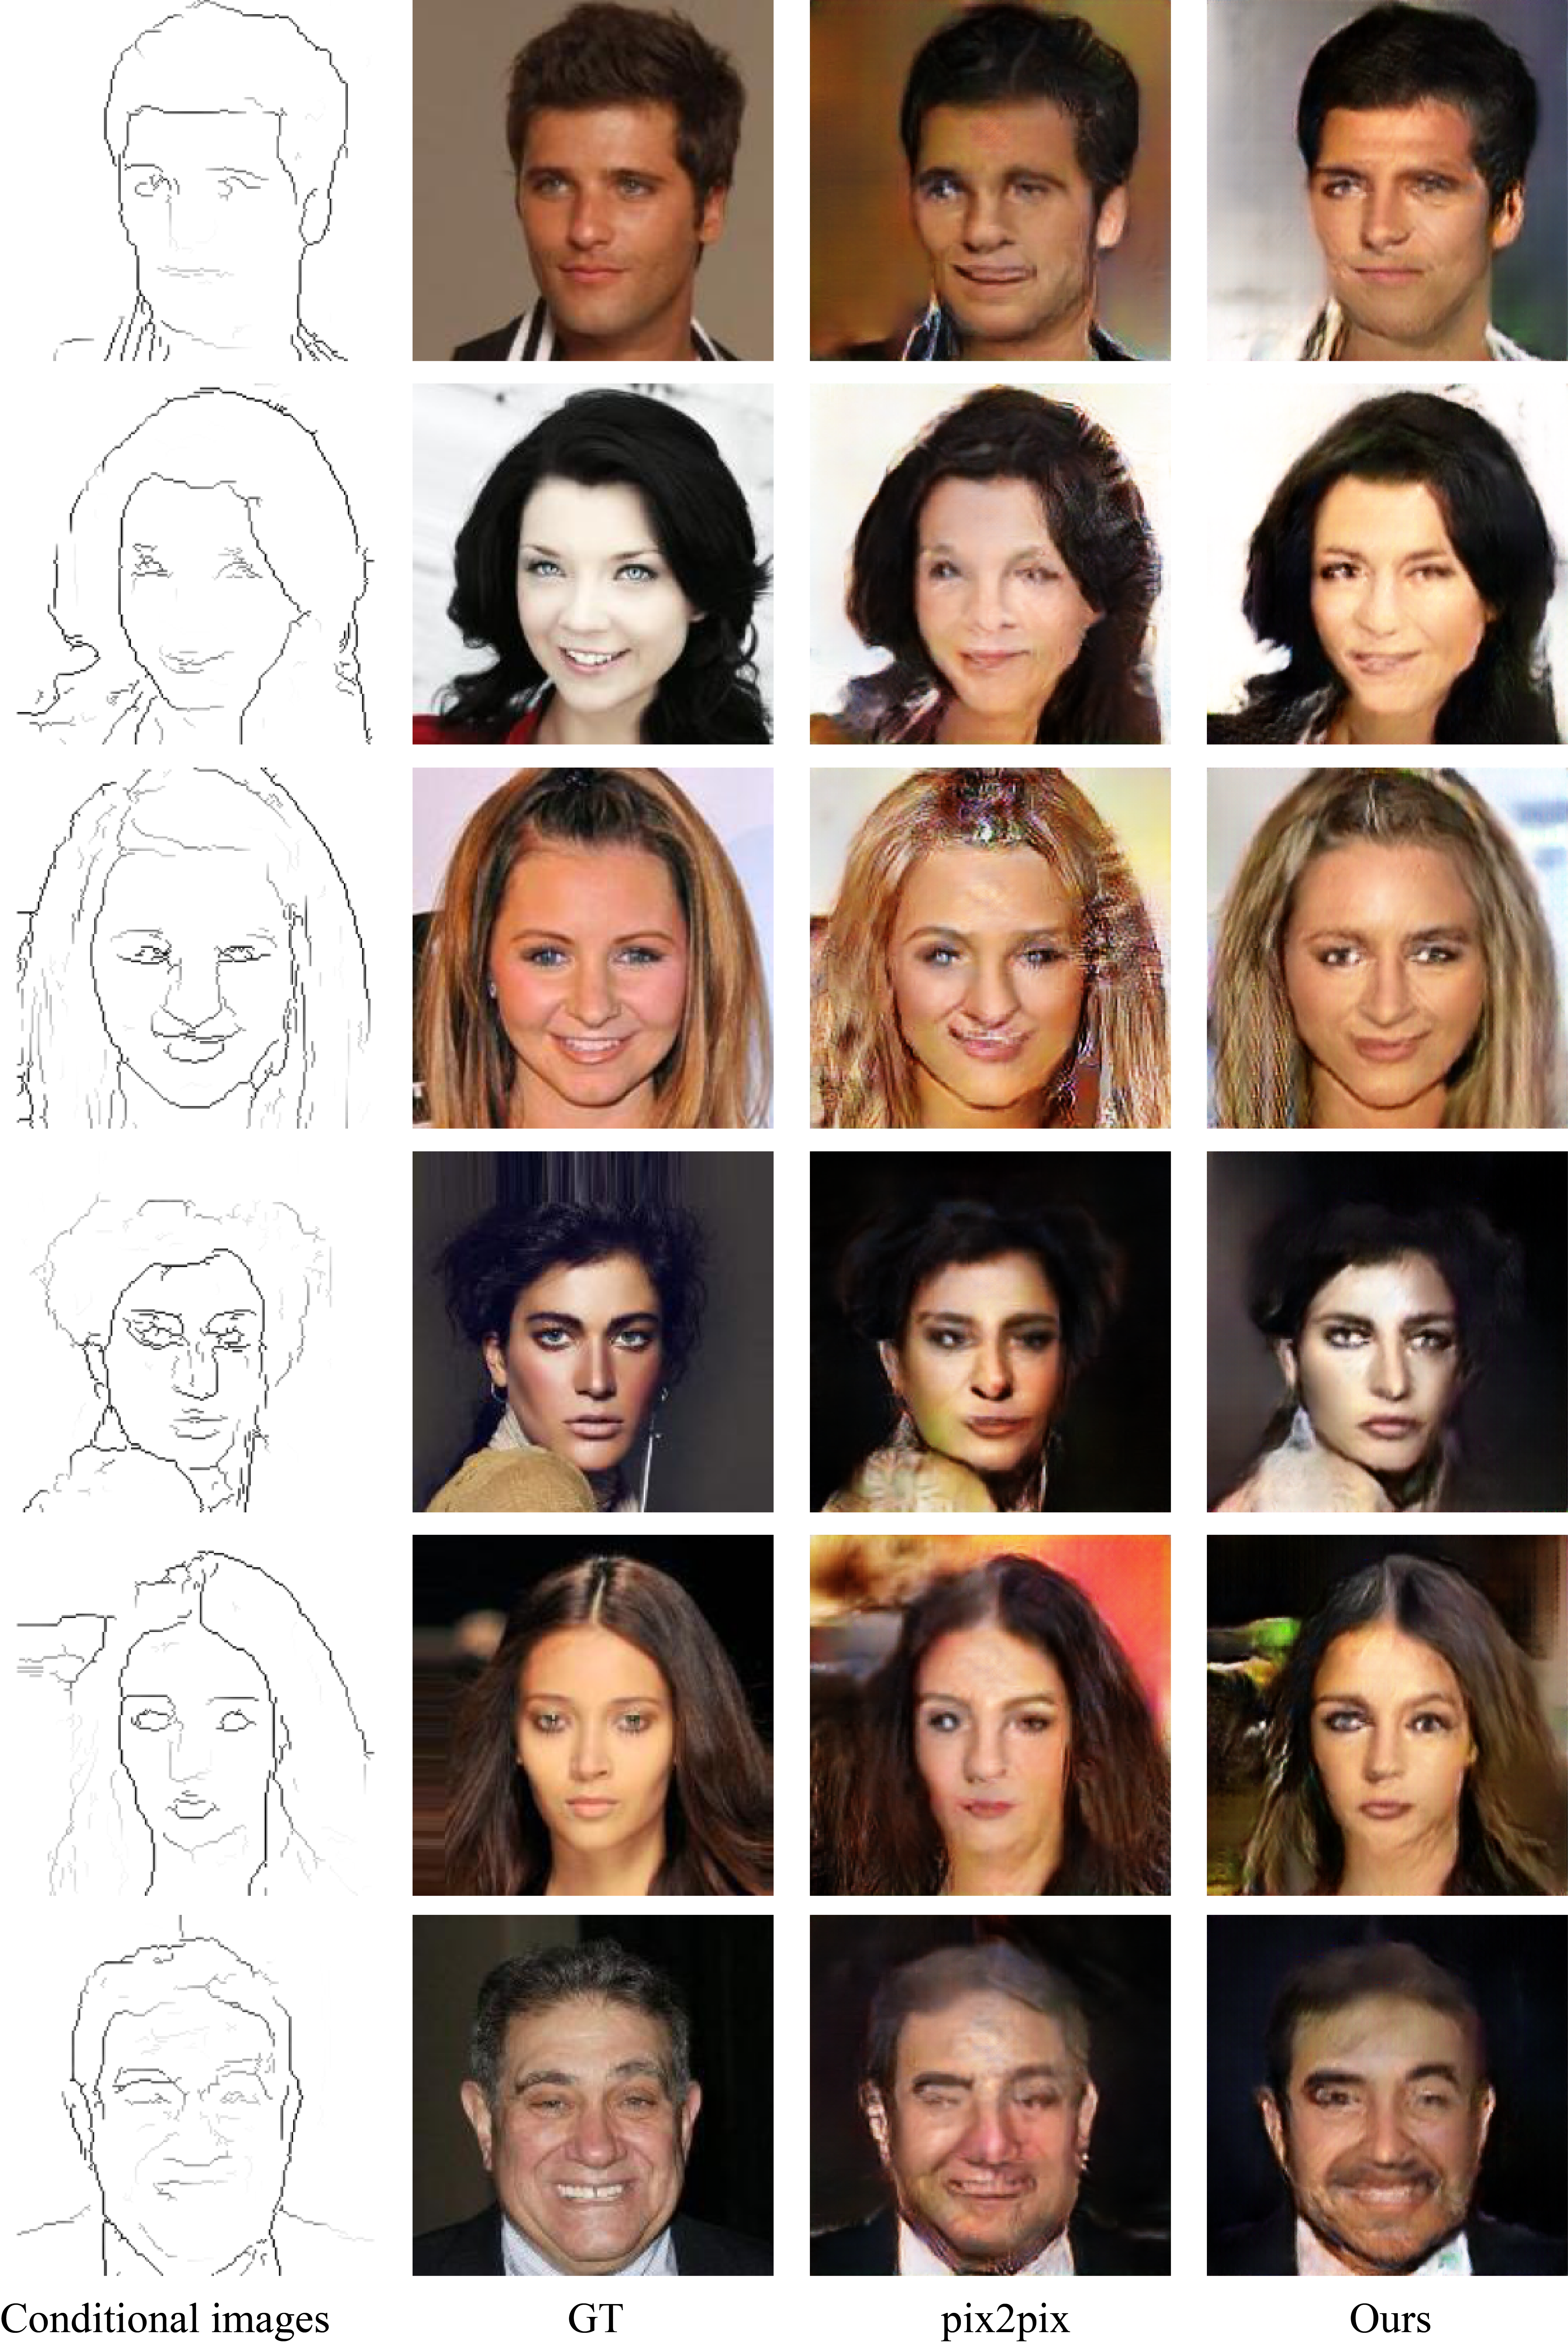
\includegraphics[width=0.8\textwidth]{figures/results}
	\caption{results}
\end{figure}
%
%
\subsection{Ablation study}

\section{Conclusion}
\label{sec:conclusion}
In this work, we introduced self-attention mechanism to the conditional GANs and proposed conditional self-attention GANs (CSAGANs). This framework is able to capture the long-range dependencies across different regions of images and global structural information. With the help of the proposed conditional self-attention module, the proposed model is able to leverage the information of conditional images directly. With a series of experiments We evaluate the effectiveness of the proposed model and advantages compared to the pix2pix model.



\end{document}
